\documentclass[a4paper,11pt,spanish,sans]{exam}
\usepackage[spanish]{babel}
%\usepackage[utf8]{inputenc}
\usepackage{multicol}
%\usepackage[latin1]{inputenc}
\usepackage{fontspec}%la posta para las tildes con lualatex
\usepackage[margin=0.5in]{geometry}
\usepackage{amsmath,amssymb}
\usepackage{multicol}
\usepackage{natbib}
\usepackage{graphicx}
\usepackage{hyperref}
\usepackage{epstopdf}
\usepackage{capt-of}
\usepackage{gensymb}
\usepackage{float}
\usepackage{wrapfig}
\usepackage{pst-fractal}
%\usepackage{animate}
\usepackage[usenames]{color}
%para graficos
\usepackage{pgf,tikz}
\usepackage{mathrsfs}
\usetikzlibrary{arrows}
\usepackage{pst-fractal}
\usetikzlibrary{decorations.markings}
\usetikzlibrary{shapes.geometric}
\usetikzlibrary{shapes,snakes}
\usepackage{tkz-euclide}
\usetkzobj{all}

\newcommand{\class}{Matemática: Integradora de 4to }
\newcommand{\term}{Diciembre 2015}
\newcommand{\examnumuno}{Tema 1\vspace{-1ex}}
\newcommand{\examnumdos}{Tema 2\vspace{-1ex}}
\newcommand{\examnumvulcano}{Tema 3\vspace{-1ex}}
\newcommand{\examprof}{Alexis Gomel\vspace{-1ex}}
\newcommand{\examdate}{20/11/2015}
\newcommand{\timelimit}{60 Minutes}%no lo uso
\newcommand{\Ts}{\rule{0pt}{2.8ex}}       % Top strut
\newcommand{\Bs}{\rule[-1.5ex]{0pt}{0pt}} % Bottom strut
%el header de las hojas.
\pagestyle{head}
\firstpageheader{}{}{}
%\runningheader{\class}{\examnumuno\ - pagina \thepage\ de \numpages}{\examdate}
%\runningheadrule
\usepackage{setspace}
\onehalfspacing

\begin{document}
	\noindent 
	\begin{minipage}{0.92\linewidth}
		\begin{tabular*}{\textwidth}{l @{\extracolsep{\fill}} r @{\extracolsep{6pt}} l}
			\textbf{\class} & \textbf{Profesor: \examprof}\\			
			\textbf{\examnumuno}  & \textbf{}   \\
			%& Teaching Assistant & %VII la venganza de adrian  \makebox[2in]{\hrulefill}
			\textbf{Nombre: } \makebox[2in]{\hrulefill} & \textbf{Fecha: } \makebox[2in]{\hrulefill}\vspace{-1ex}
		\end{tabular*}\\
	\end{minipage}
	\begin{minipage}[r]{0.08\linewidth}
		\begin{flushright}
			
\includegraphics[width=\linewidth]{bost.png}
		\end{flushright}
	\end{minipage}\\
	\rule[2ex]{\textwidth, \vspace{-2ex}}{2pt}
\begin{center}
	\textsl{\textbf{\underline{Justificar}}} cada respuesta. La evaluación se entrega \textbf{\underline{escrita en tinta}}.\\
	Si se traban con un ejercicio sigan con el siguiente.
	May the force be with you.\vspace{-2ex}
\end{center}
\begin{table}[h]
	\centering
	%\caption{My caption}
	\label{tema1}
	\begin{tabular}{|l|c|c|c|c|c||}
		\hline
		Ejercicio        & 1 & 2 & 3 & Nota & Hojas \\ \hline
		Puntaje máximo   & 4 & 3 & 3 & 10 &  Entregadas \\ \hline
		Puntaje obtenido &   &   &   &    &   \\ \hline 
	\end{tabular}
\end{table}
\section{Trigonometria (4 puntos)\vspace{-2ex}}
Resolver los siguientes triángulos (Calcular los lados, los ángulos y sus razones trigonométricas). \label{rectangulos1}\\

	\begin{minipage}{0.5\linewidth}
		
		\begin{tikzpicture}[thick]
		\coordinate (O) at (0,0);
		\coordinate (A) at (3.5,0);
		\coordinate (B) at (0,2.6);
		\draw (O)--(A)--(B)--cycle;
		
		\tkzLabelSegment[below=2pt](O,A){$b$}
		\tkzLabelSegment[left=2pt](O,B){$a=5cm$}
		\tkzLabelSegment[above right=2pt](A,B){$h=13$}
		
		\tkzMarkRightAngle[fill=orange,size=0.6,opacity=.4](A,O,B)% square angle here
		\tkzLabelAngle[pos = 0.35](A,O,B){$\hat{\gamma}$}
		
		\tkzMarkAngle[fill= orange,size=0.8cm,%
		opacity=.4](B,A,O)
		\tkzLabelAngle[pos = 0.6](B,A,O){$\hat{\alpha}$}
		
		\tkzMarkAngle[fill= orange,size=0.8cm,%
		opacity=.4](O,B,A)
		\tkzLabelAngle[pos = 0.5](O,B,A){$\hat{\beta}$}
		
		\end{tikzpicture}
	\end{minipage}
%	\begin{minipage}{0.55\linewidth}
%		\begin{enumerate}
%			%\item $a=3km$,  $\quad b=4km$ .	Expresar los resultados de los ángulos en el sistema sexagesimal.
%			\item $a=5cm$, $\quad h=13cm$
%			
%			%\item $a=2cm$, $\quad b=1cm$
%			%\item $a=30km$,  $\quad b=20km$ .	Expresar los resultados de los ángulos en el sistema sexagesimal.
%			%\item $a=5cm$, $\quad \sin(\beta)=\frac{1}{\sqrt{2}}$. Expresar los resultados de los ángulos en Radianes.
%			%\item $a=5cm$, $\quad \cos(\alpha)=\frac{\sqrt{2}}{2}$
%%			\item $a=5cm$, $\quad \cos(\alpha)=\frac{\sqrt{3}}{2}$ 
%
%		\end{enumerate}
%	\end{minipage}
%Encontrar los restantes y los ángulos internos.
\begin{minipage}{0.45\linewidth}
\begin{tikzpicture}[thick]
\coordinate (O) at (0,0);
\coordinate (A) at (2.5,0);
\coordinate (B) at (4.5,1.5);
\draw (O)--(A)--(B)--cycle;

\tkzLabelSegment[below=2pt](O,A){}
\tkzLabelSegment[left=2pt](O,B){$37km$}
\tkzLabelSegment[above right=2pt](A,B){}

\tkzMarkAngle[fill=orange,size=0.3cm,opacity=.4](A,O,B)
\tkzLabelAngle[pos = -0.7](A,O,B){$\hat{\gamma}=30\degree $}

\tkzMarkAngle[fill= orange,size=0.3cm,%
opacity=.4](B,A,O)
\tkzLabelAngle[ pos= -0.4 ](B,A,O){$\hat{\alpha}=140\degree$}

\tkzMarkAngle[fill= orange,size=0.3cm,opacity=.4](O,B,A)
\tkzLabelAngle[pos = -0.4](O,B,A){}
\end{tikzpicture}
\end{minipage}

\section{Complejos (3 puntos)\vspace{-2ex}}
\begin{multicols}{2}
\begin{enumerate}
			Dados $\quad z_1=2-i$ ;  $\quad z_2=-2+3i$ ;  $\quad z_3=1-i$\\
			
			Calcular:\\ 
			
			\item $|z_1|^2+\left(  \dfrac{z_2}{z_3} \right) ^{-1}$\\
			
			\item $z_1+z_1^*$\\
			
			\columnbreak
					
			\\Resolver la siguiente ecuación y graficar el resultado en el plano complejo.\\
			\item $(-\frac{1}{2}x+3;-y+\frac{1}{4})=(0; 1)$	
\end{enumerate}
\end{multicols}

	
\section{Funciones Racionales (3 puntos)}
%Graficar $y=-\dfrac{5(x+1)(x-1)}{(x-3)}$
	\begin{minipage}{0.5\textwidth}
		\centering
		%\begin{table}[!h]
		%\caption{mc1}
		\label{mc1}
		\begin{tabular}{|c|c|c|}
			\hline
				$\dfrac{5x^4}{(x-3)^3(x-1)}$  & $\dfrac{x^4(x-3)^3}{(x-1)}$ & $\dfrac{x^4}{5(x-3)^3(x+1)}$ \Ts \Bs   \\
			&   &      \\ \hline
		\end{tabular}\\
		%\end{table}
		%\begin{figure}[h]
		\centering
		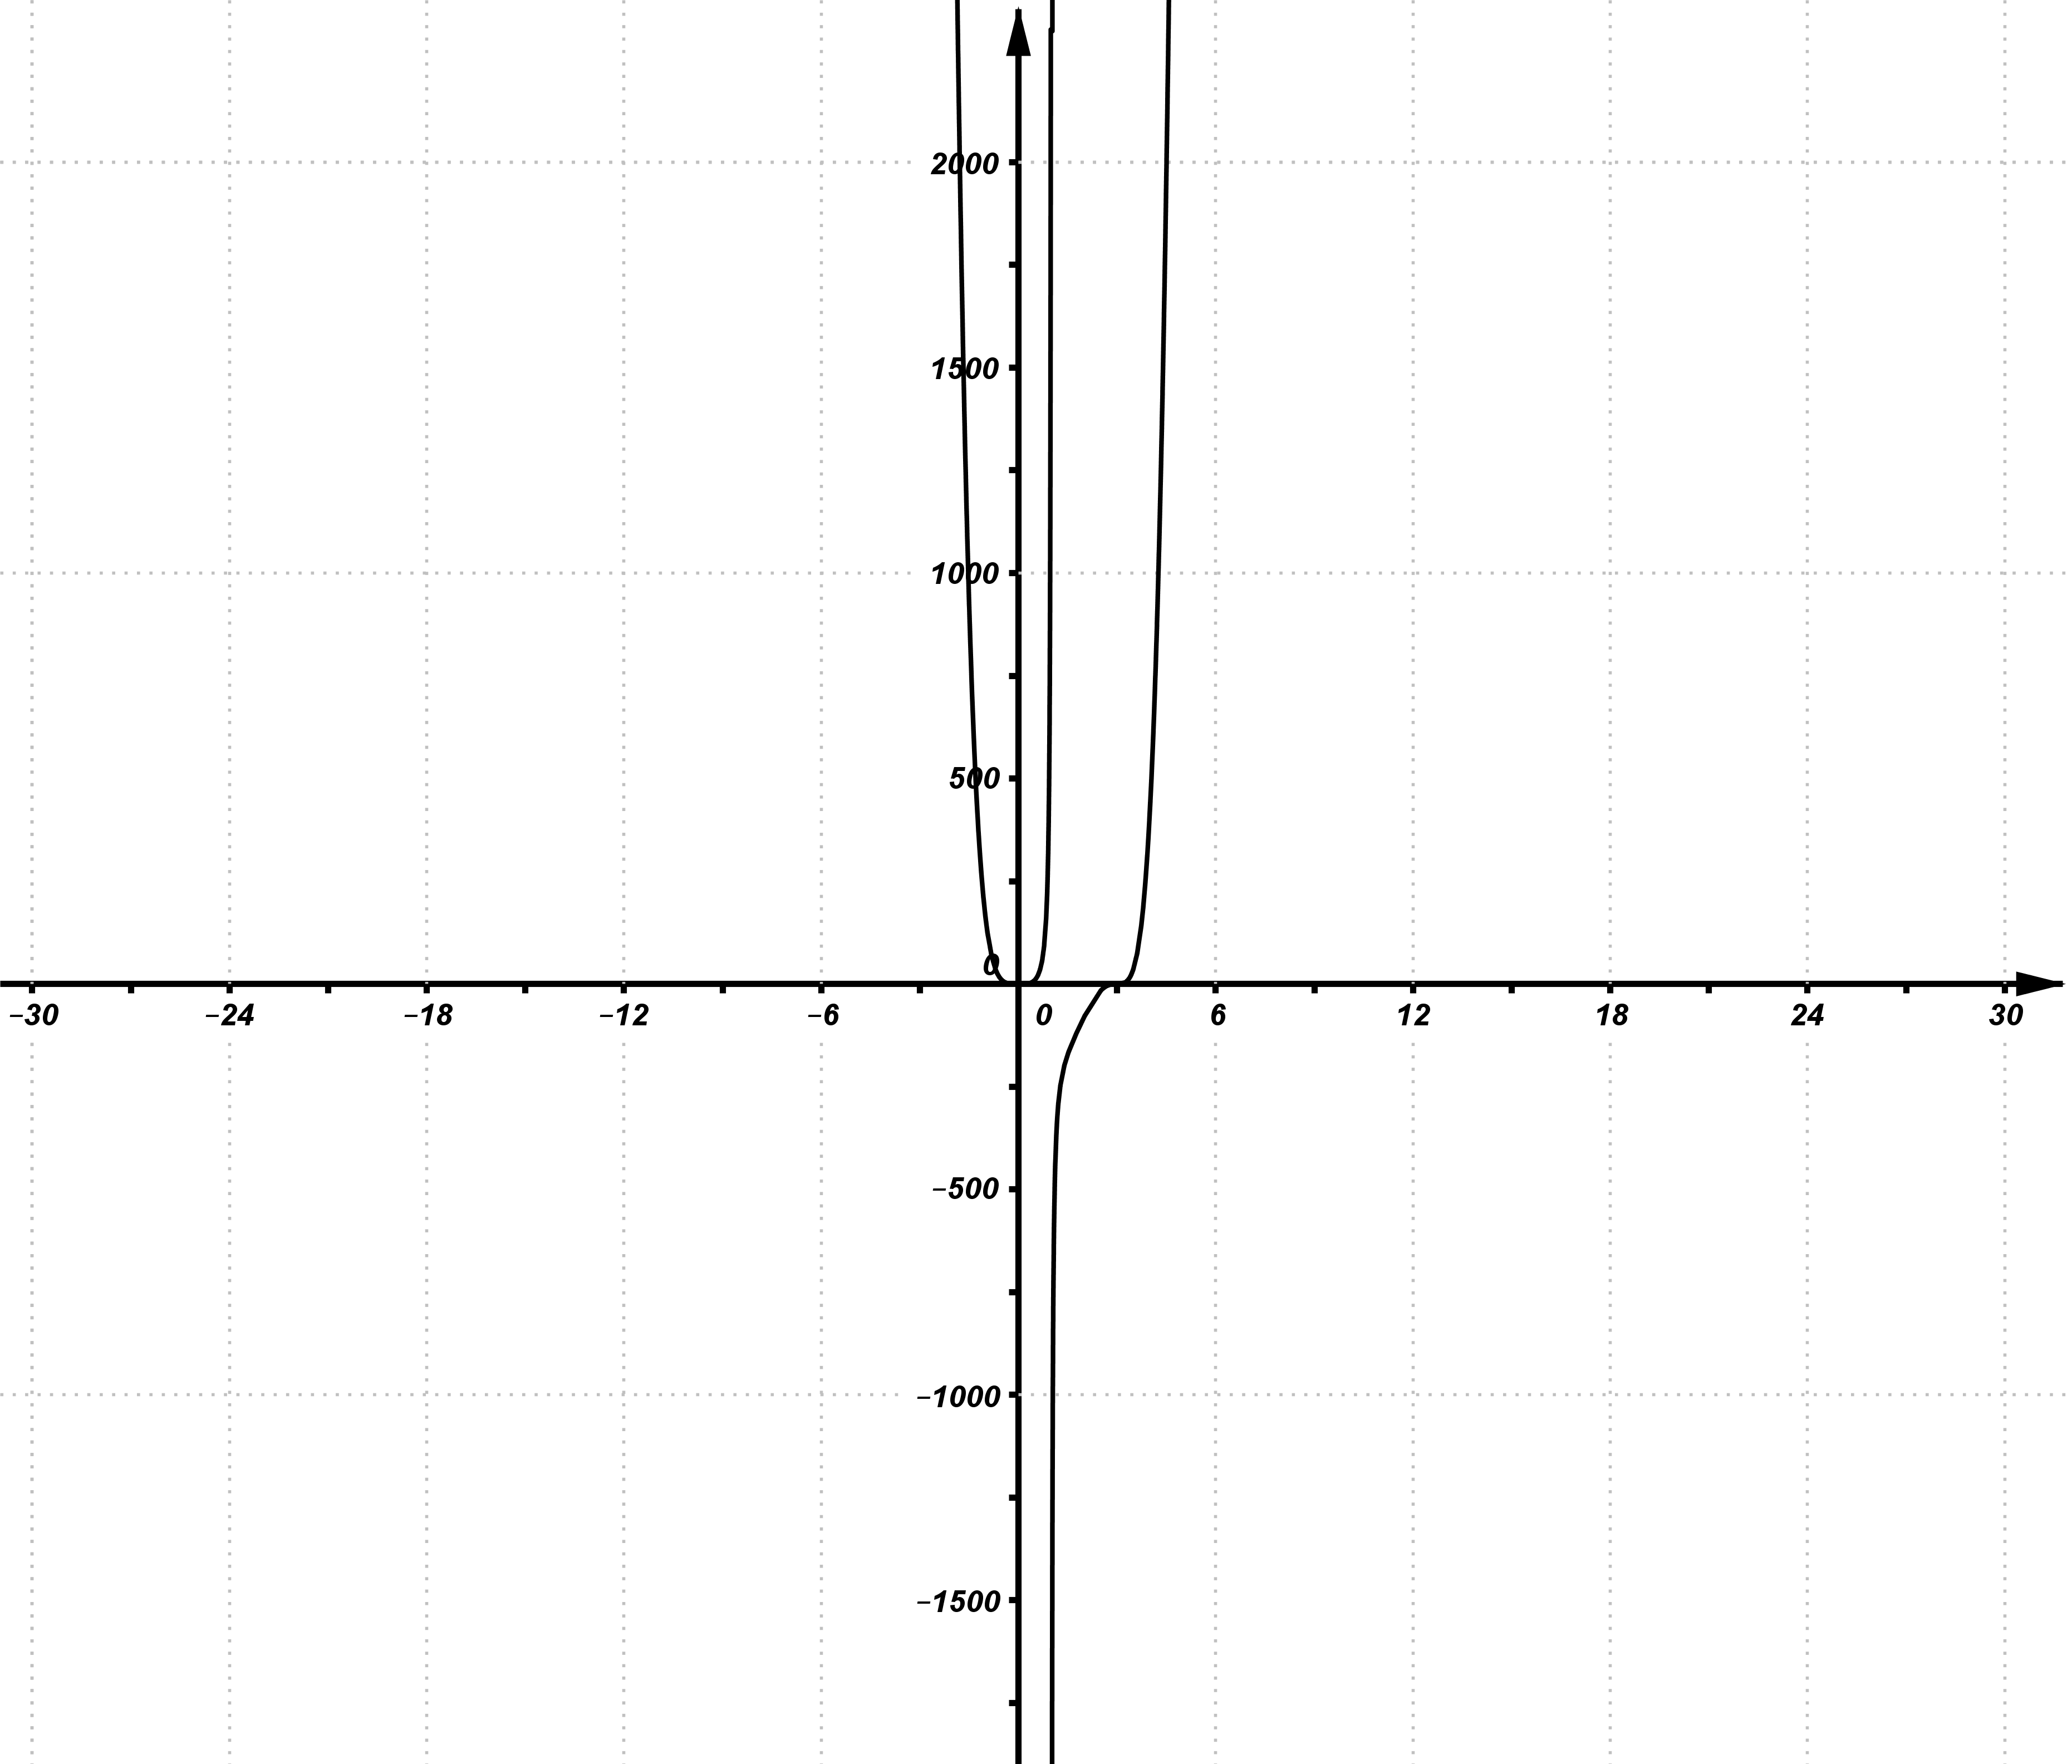
\includegraphics[width= 0.95\linewidth]{2dadic.png}
		%\end{figure}
		%graficos
	\end{minipage}
	\begin{minipage}{.5\textwidth}
		\centering
		%\begin{table}[!h]
		%\caption{mc1}
		%\label{mc1}
		\begin{tabular}{|c|c|c|}
			\hline
			$\dfrac{2(x-1)^2(x+1)}{x}$  & $\dfrac{x}{(x+1)(x+1)}$ & $\dfrac{2(x-1)(x+1)}{x}$ \Ts \Bs   \\ \hline
			&   &      \\ \hline
		\end{tabular}\\
		%\end{table}
		%\begin{figure}[h]
		\centering
		
\includegraphics[width= 0.95\linewidth]{dadic4.png}
		%\end{figure}
	\end{minipage}\\
2. Encontrar todos los valores de $x$ tal que: $\dfrac{3x-1}{x+2}<2$

\setcounter{section}{0}

\newpage

	\noindent 
	\begin{minipage}{0.92\linewidth}
		\begin{tabular*}{\textwidth}{l @{\extracolsep{\fill}} r @{\extracolsep{6pt}} l}
			\textbf{\class} & \textbf{Profesor: \examprof}\\			
			\textbf{\examnumdos}  & \textbf{}   \\
			%& Teaching Assistant & %VII la venganza de adrian  \makebox[2in]{\hrulefill}
			\textbf{Nombre: } \makebox[2in]{\hrulefill} & \textbf{Fecha: } \makebox[2in]{\hrulefill}\vspace{-1ex}
		\end{tabular*}\\
	\end{minipage}
	\begin{minipage}[r]{0.08\linewidth}
		\begin{flushright}
			
\includegraphics[width=\linewidth]{bost.png}
		\end{flushright}
	\end{minipage}\\
	\rule[2ex]{\textwidth, \vspace{-2ex}}{2pt}
	\begin{center}
		\textsl{\textbf{\underline{Justificar}}} cada respuesta. La evaluación se entrega \textbf{\underline{escrita en tinta}}.\\
		Si se traban con un ejercicio sigan con el siguiente.
		May the force be with you.\vspace{-2ex}
	\end{center}
	\begin{table}[h]
		\centering
		%\caption{My caption}
		\label{tema2}
		\begin{tabular}{|l|c|c|c|c|c||}
			\hline
			Ejercicio        & 1 & 2 & 3 & Nota & Hojas \\ \hline
			Puntaje máximo   & 4 & 3 & 3 & 10 &  Entregadas \\ \hline
			Puntaje obtenido &   &   &   &    &   \\ \hline 
		\end{tabular}
	\end{table}
	\section{Trigonometria (4 puntos)\vspace{-2ex}}
	Resolver los siguientes triángulos (Calcular los lados, los ángulos y sus razones trigonométricas). \label{rectangulos2}\\
	
	\begin{minipage}{0.5\linewidth}
		
		\begin{tikzpicture}[thick]
		\coordinate (O) at (0,0);
		\coordinate (A) at (3.5,0);
		\coordinate (B) at (0,2.6);
		\draw (O)--(A)--(B)--cycle;
		
		\tkzLabelSegment[below=2pt](O,A){$b=20cm$}
		\tkzLabelSegment[left=2pt](O,B){$a=12cm$}
		\tkzLabelSegment[above right=2pt](A,B){$h$}
		
		\tkzMarkRightAngle[fill=orange,size=0.6,opacity=.4](A,O,B)% square angle here
		\tkzLabelAngle[pos = 0.35](A,O,B){$\hat{\gamma}$}
		
		\tkzMarkAngle[fill= orange,size=0.8cm,%
		opacity=.4](B,A,O)
		\tkzLabelAngle[pos = 0.6](B,A,O){$\hat{\alpha}$}
		
		\tkzMarkAngle[fill= orange,size=0.8cm,%
		opacity=.4](O,B,A)
		\tkzLabelAngle[pos = 0.5](O,B,A){$\hat{\beta}$}
		
		\end{tikzpicture}
	\end{minipage}
	%	\begin{minipage}{0.55\linewidth}
	%		\begin{enumerate}
	%			%\item $a=3km$,  $\quad b=4km$ .	Expresar los resultados de los ángulos en el sistema sexagesimal.
	%			\item $a=5cm$, $\quad h=13cm$
	%			
	%			%\item $a=2cm$, $\quad b=1cm$
	%			%\item $a=30km$,  $\quad b=20km$ .	Expresar los resultados de los ángulos en el sistema sexagesimal.
	%			%\item $a=5cm$, $\quad \sin(\beta)=\frac{1}{\sqrt{2}}$. Expresar los resultados de los ángulos en Radianes.
	%			%\item $a=5cm$, $\quad \cos(\alpha)=\frac{\sqrt{2}}{2}$
	%%			\item $a=5cm$, $\quad \cos(\alpha)=\frac{\sqrt{3}}{2}$ 
	%
	%		\end{enumerate}
	%	\end{minipage}
	%Encontrar los restantes y los ángulos internos.
	\begin{minipage}{0.45\linewidth}
		\begin{tikzpicture}[thick]
		\coordinate (O) at (0,0);
		\coordinate (A) at (2.5,0);
		\coordinate (B) at (4,1.9);
		\draw (O)--(A)--(B)--cycle;
		
		\tkzLabelSegment[below=2pt](O,A){$15$}
		\tkzLabelSegment[left=2pt](O,B){}
		\tkzLabelSegment[center below=4pt](A,B){$38$}
		
		\tkzMarkAngle[fill=orange,size=0.3cm,opacity=.4](A,O,B)
		\tkzLabelAngle[pos = -0.7](A,O,B){}
		
		\tkzMarkAngle[fill= orange,size=0.3cm,
		opacity=.4](B,A,O)
		\tkzLabelAngle[ pos= -0.4 ](B,A,O){$\hat{\alpha}=100\degree$}
		
		\tkzMarkAngle[fill= orange,size=0.3cm,opacity=.4](O,B,A)
		\tkzLabelAngle[pos = -0.4](O,B,A){}
		\end{tikzpicture}
	\end{minipage}
	
	\section{Complejos (3 puntos)\vspace{-2ex}}
	\begin{multicols}{2}
		\begin{enumerate}
			Dados $\quad z_1=2-i$ ;  $\quad z_2=-2+3i$ ;  $\quad z_3=1-i$\\
			
			Calcular:\\ 
			
						\item $\dfrac{z_1}{z_2.z_3}$\\
			
				\item $\dfrac{z_2^2+|z_{3}|^2}{z_1^*}$\\
			
			\columnbreak
			
			\\Resolver la siguiente ecuación y graficar el resultado en el plano complejo.\\
	\item $3x-1+(1-y)i=(2;3)$
		\end{enumerate}
	\end{multicols}
	
	
	\section{Funciones Racionales (3 puntos)}
	%Graficar $y=-\dfrac{5(x+1)(x-1)}{(x-3)}$
	\begin{minipage}{0.5\textwidth}
		\centering
		%\begin{table}[!h]
		%\caption{mc1}
		\label{mc2}
		\begin{tabular}{|c|c|c|}
			\hline
			$\dfrac{2(x-1)^2(x+1)}{x}$  & $\dfrac{x}{(x+1)(x+1)}$ & $\dfrac{2(x-1)(x+1)}{x}$ \Ts \Bs   \\ \hline
				&   &      \\ \hline
		\end{tabular}\\
		%\end{table}
		%\begin{figure}[h]
		\centering
		
\includegraphics[width= 0.95\linewidth]{2dadic2.png}
		%\end{figure}
		%graficos
	\end{minipage}
	\begin{minipage}{.5\textwidth}
		\centering
		%\begin{table}[!h]
		%\caption{mc1}
		%\label{mc1}
		\begin{tabular}{|c|c|c|}
			\hline
			$\dfrac{5x^4}{(x-3)^3(x-1)}$  & $\dfrac{x^4(x-3)^3}{(x-1)}$ & $\dfrac{x^4}{5(x-3)^3(x+1)}$ \Ts \Bs   \\ \hline
			&   &      \\ \hline
		\end{tabular}\\
		%\end{table}
		%\begin{figure}[h]
		\centering
		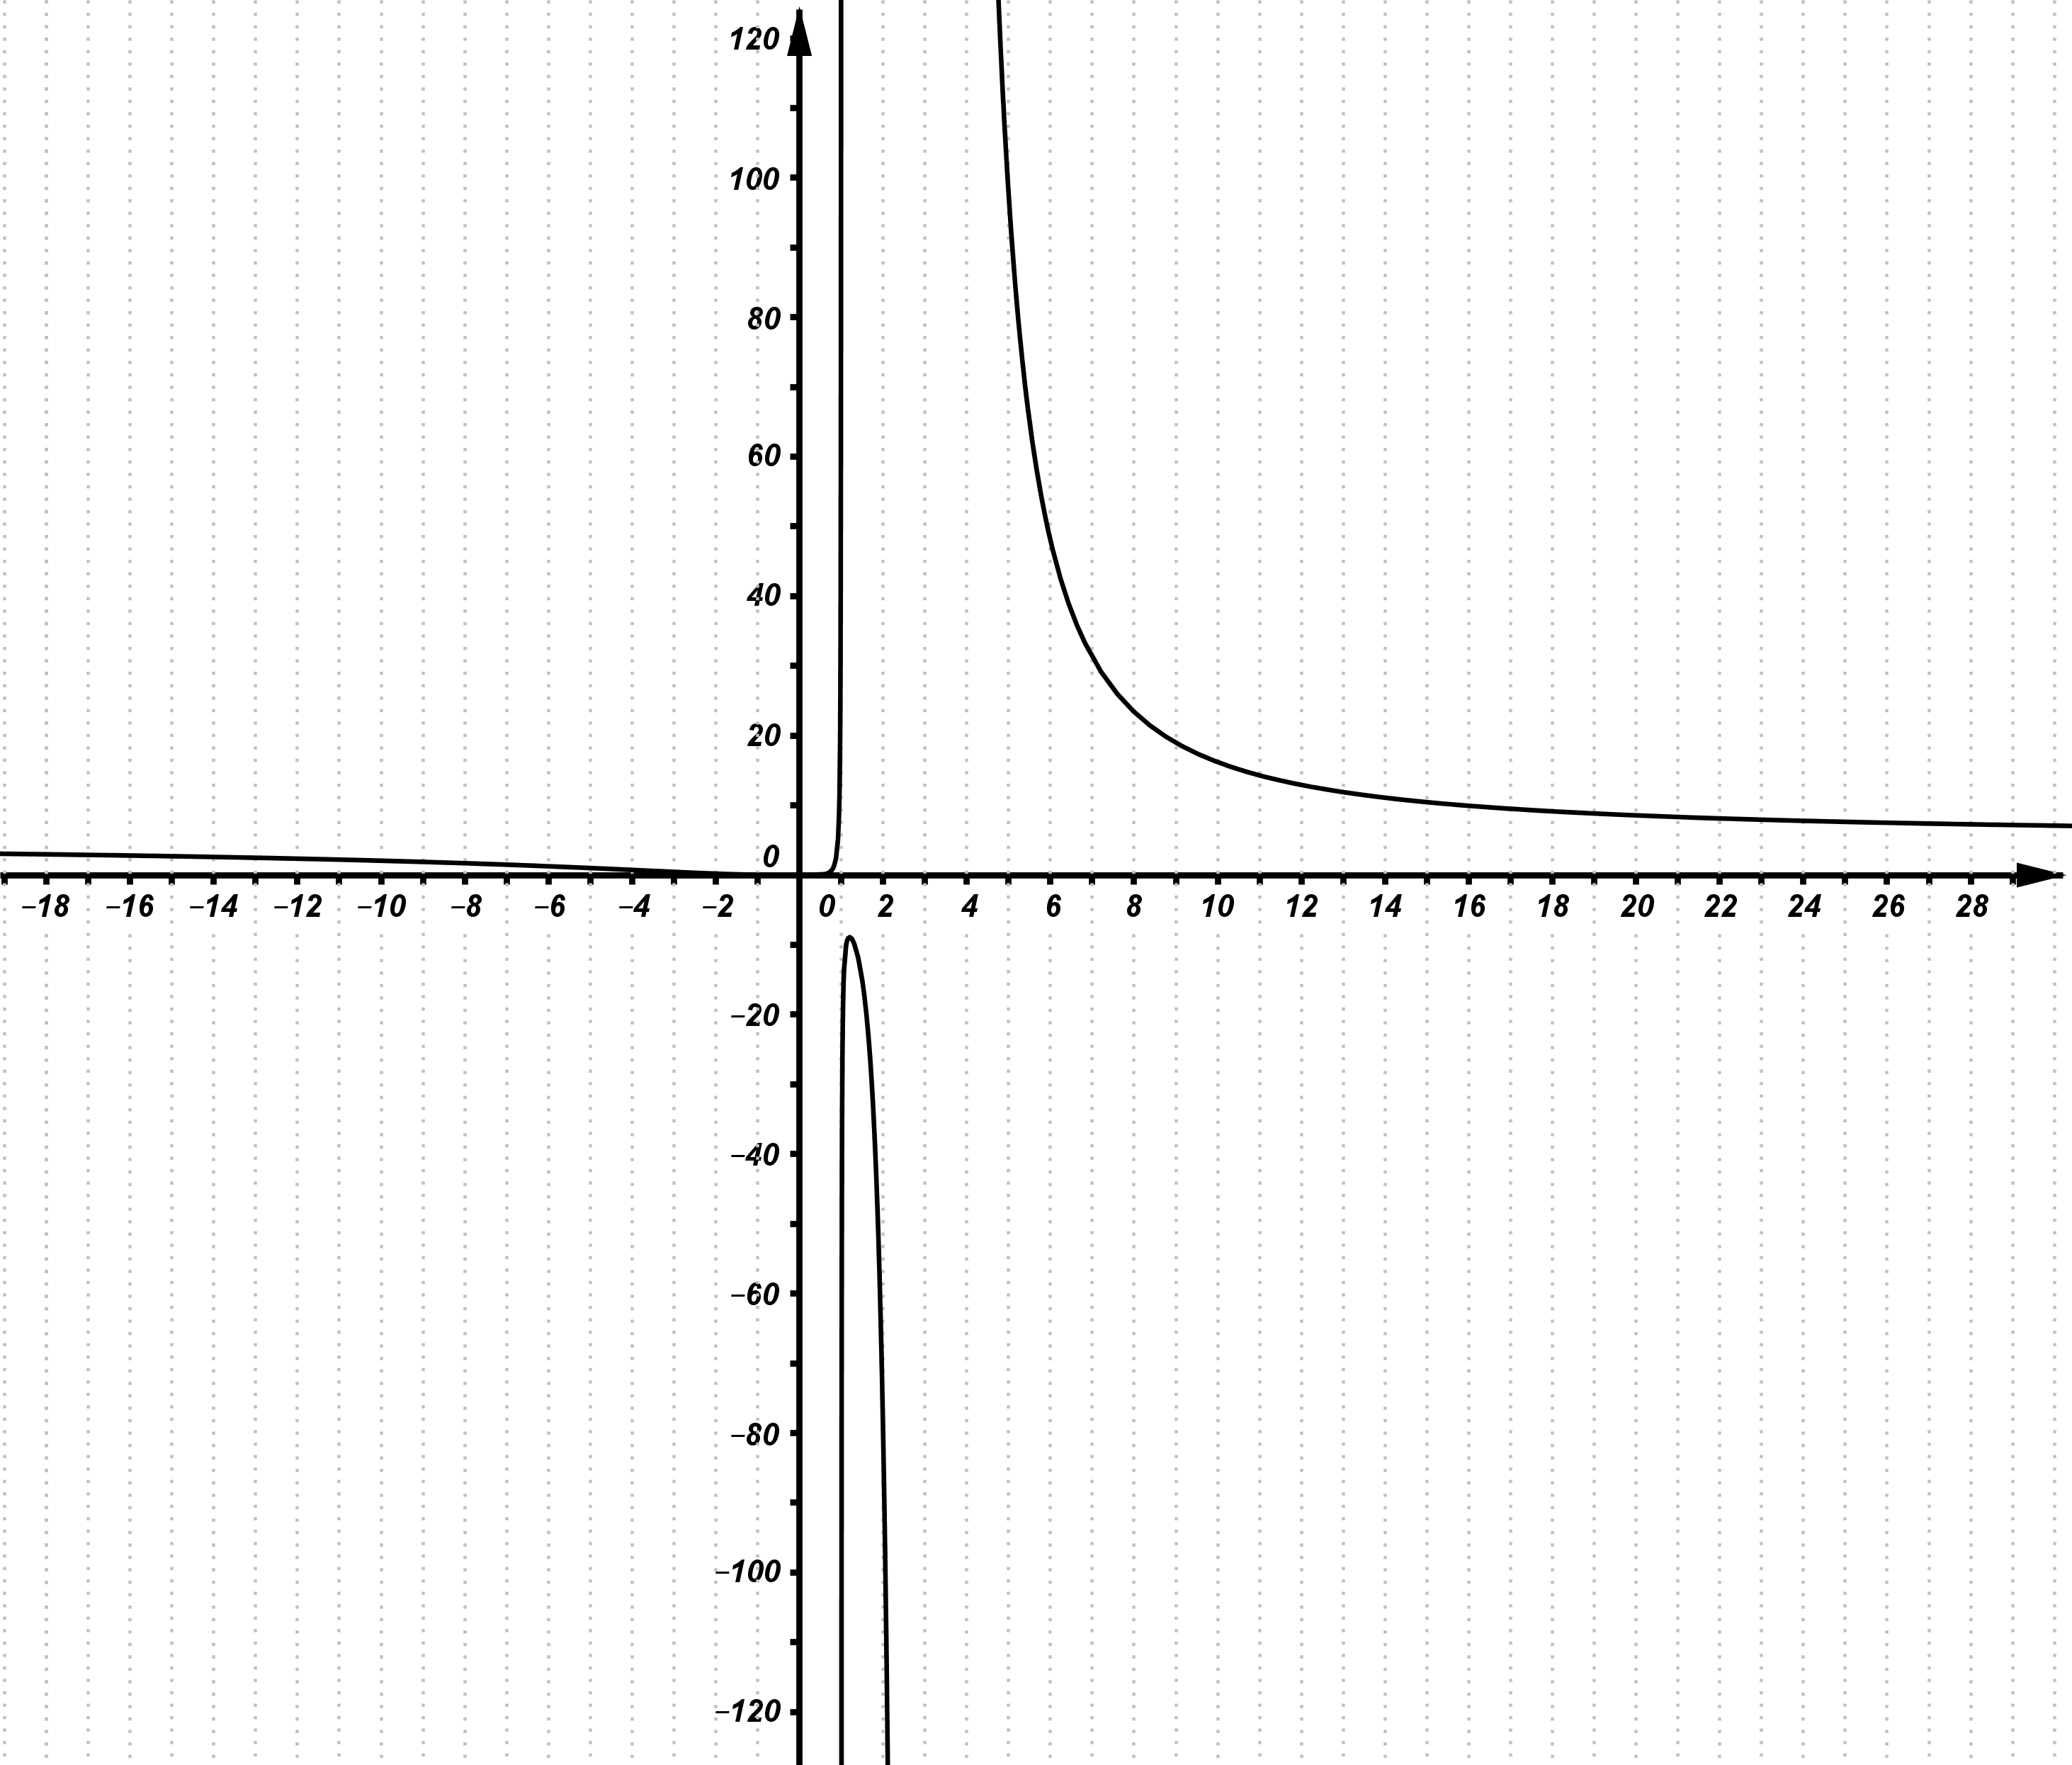
\includegraphics[width= 0.95\linewidth]{2dadic3.png}
		%\end{figure}
	\end{minipage}\\
	2. Encontrar todos los valores de $x$ tal que: $\dfrac{3x-1}{x+2}>2$

\setcounter{section}{0}

\newpage

	\noindent 
	\begin{minipage}{0.92\linewidth}
		\begin{tabular*}{\textwidth}{l @{\extracolsep{\fill}} r @{\extracolsep{6pt}} l}
			\textbf{\class} & \textbf{Profesor: \examprof}\\			
			\textbf{\examnumvulcano}  & \textbf{}   \\
			%& Teaching Assistant & %VII la venganza de adrian  \makebox[2in]{\hrulefill}
			\textbf{Nombre: } \makebox[2in]{\hrulefill} & \textbf{Fecha: } \makebox[2in]{\hrulefill}\vspace{-1ex}
		\end{tabular*}\\
	\end{minipage}
	\begin{minipage}[r]{0.08\linewidth}
		\begin{flushright}
			
\includegraphics[width=\linewidth]{bost.png}
		\end{flushright}
	\end{minipage}\\
	\rule[2ex]{\textwidth, \vspace{-2ex}}{2pt}
	\begin{center}
		\textsl{\textbf{\underline{Justificar}}} cada respuesta. La evaluación se entrega \textbf{\underline{escrita en tinta}}.\\
		Si se traban con un ejercicio sigan con el siguiente.
		May the force be with you.\vspace{-2ex}
	\end{center}
	\begin{table}[h]
		\centering
		%\caption{My caption}
		\label{tema3}
		\begin{tabular}{|l|c|c|c|c|c||}
			\hline
			Ejercicio        & 1 & 2 & 3 & Nota & Hojas \\ \hline
			Puntaje máximo   & 4 & 3 & 3 & 10 &  Entregadas \\ \hline
			Puntaje obtenido &   &   &   &    &   \\ \hline 
		\end{tabular}
	\end{table}
	\section{Trigonometria (4 puntos)\vspace{-2ex}}
	Resolver los siguientes triángulos (Calcular los lados, los ángulos y sus razones trigonométricas). \label{rectangulos3}\\
	
	\begin{minipage}{0.5\linewidth}
		
		\begin{tikzpicture}[thick]
		\coordinate (O) at (0,0);
		\coordinate (A) at (3.5,0);
		\coordinate (B) at (0,2.6);
		\draw (O)--(A)--(B)--cycle;
		
		\tkzLabelSegment[below=2pt](O,A){$b=20cm$}
		\tkzLabelSegment[left=2pt](O,B){$a=12cm$}
		\tkzLabelSegment[above right=2pt](A,B){$h$}
		
		\tkzMarkRightAngle[fill=orange,size=0.6,opacity=.4](A,O,B)% square angle here
		\tkzLabelAngle[pos = 0.35](A,O,B){$\hat{\gamma}$}
		
		\tkzMarkAngle[fill= orange,size=0.8cm,%
		opacity=.4](B,A,O)
		\tkzLabelAngle[pos = 0.6](B,A,O){$\hat{\alpha}$}
		
		\tkzMarkAngle[fill= orange,size=0.8cm,%
		opacity=.4](O,B,A)
		\tkzLabelAngle[pos = 0.5](O,B,A){$\hat{\beta}$}
		
		\end{tikzpicture}
	\end{minipage}
	%	\begin{minipage}{0.55\linewidth}
	%		\begin{enumerate}
	%			%\item $a=3km$,  $\quad b=4km$ .	Expresar los resultados de los ángulos en el sistema sexagesimal.
	%			\item $a=5cm$, $\quad h=13cm$
	%			
	%			%\item $a=2cm$, $\quad b=1cm$
	%			%\item $a=30km$,  $\quad b=20km$ .	Expresar los resultados de los ángulos en el sistema sexagesimal.
	%			%\item $a=5cm$, $\quad \sin(\beta)=\frac{1}{\sqrt{2}}$. Expresar los resultados de los ángulos en Radianes.
	%			%\item $a=5cm$, $\quad \cos(\alpha)=\frac{\sqrt{2}}{2}$
	%%			\item $a=5cm$, $\quad \cos(\alpha)=\frac{\sqrt{3}}{2}$ 
	%
	%		\end{enumerate}
	%	\end{minipage}
	%Encontrar los restantes y los ángulos internos.
	\begin{minipage}{0.45\linewidth}
		\begin{tikzpicture}[thick]
		\coordinate (O) at (0,0);
		\coordinate (A) at (2.5,0);
		\coordinate (B) at (4,1.9);
		\draw (O)--(A)--(B)--cycle;
		
		\tkzLabelSegment[below=2pt](O,A){$15$}
		\tkzLabelSegment[left=2pt](O,B){}
		\tkzLabelSegment[center below=2pt](A,B){$38$}
		
		\tkzMarkAngle[fill=orange,size=0.3cm,opacity=.4](A,O,B)
		\tkzLabelAngle[pos = -0.7](A,O,B){}
		
		\tkzMarkAngle[fill= orange,size=0.3cm,%
		opacity=.4](B,A,O)
		\tkzLabelAngle[ pos= -0.4 ](B,A,O){$\hat{\alpha}=100\degree$}
		
		\tkzMarkAngle[fill= orange,size=0.3cm,opacity=.4](O,B,A)
		\tkzLabelAngle[pos = -0.4](O,B,A){}
		\end{tikzpicture}
	\end{minipage}
	
	\section{Complejos (3 puntos)\vspace{-2ex}}
	\begin{multicols}{2}
		\begin{enumerate}
			
			
			Calcular:\\ 
		
		\item $\dfrac{(-1+i)+(2-4i)}{-2+3i}$\\
		
		\item $\dfrac{(1+i)^2}{1-i}$
			
			\columnbreak
			
			\\Resolver la siguiente ecuación y graficar el resultado en el plano complejo.\\
	\item $x+(1-y)i=(2;3)$
	\end{enumerate}
	\end{multicols}
	
	
	\section{Funciones Racionales (3 puntos)}
	%Graficar $y=-\dfrac{5(x+1)(x-1)}{(x-3)}$
	\begin{minipage}{0.5\textwidth}
		\centering
		%\begin{table}[!h]
		%\caption{mc1}
		\label{mc3}
		\begin{tabular}{|c|c|c|}
			\hline
			$x^2$  & $\dfrac{1}{x^2}$ & $\dfrac{1}{x}$ \Ts \Bs   \\ \hline
			&   &      \\ \hline
		\end{tabular}\\
		%\end{table}
		%\begin{figure}[h]
		\centering
		
\includegraphics[width= 0.95\linewidth]{didacvulcano.png}
		%\end{figure}
		%graficos
	\end{minipage}
	\begin{minipage}{.5\textwidth}
		\centering
		%\begin{table}[!h]
		%\caption{mc1}
		%\label{mc1}
		\begin{tabular}{|c|c|c|}
			\hline
			$\dfrac{x^2}{(x-1)}$  & $\dfrac{x^2}{(x+1)}$ & $\dfrac{x+1}{x^2}$ \Ts \Bs   \\ \hline
			&   &      \\ \hline
		\end{tabular}\\
		%\end{table}
		%\begin{figure}[h]
		\centering
		
\includegraphics[width= 0.95\linewidth]{didacvulcano2.png}
		%\end{figure}
	\end{minipage}\\
	2. Encontrar todos los valores de $x$ tal que: $\dfrac{x}{x+2}<2$
	



\end{document}